% Practice Test 18 — Indiana Edition
% Questions: 30 (26 MC + 4 SA)
% Generated by scripts/generate_practice_tests.py

\begin{practiceQuestion}{1-3-q12}{mc}
\begin{questionText}
A proportional table has $k = \frac{3}{4}$. Which pair could be in the table?
\end{questionText}
\choiceA{$(8, 10)$}
\choiceB{$(8, 6)$}
\choiceC{$(12, 8)$}
\choiceD{$(4, 2)$}
\correctAnswer{B}
\explanation{If $k = \frac{3}{4}$, then $y = \frac{3}{4}x$. For $x = 8$: $y = \frac{3}{4} \times 8 = 6$. So $(8, 6)$ works.}
\end{practiceQuestion}

\begin{practiceQuestion}{1-5-q04}{mc}
\begin{questionText}
Two proportional lines are graphed. Line A is steeper than Line B. What does this tell you?
\end{questionText}
\choiceA{Line A has a smaller unit rate}
\choiceB{Line A has a greater unit rate}
\choiceC{Line B covers more distance}
\choiceD{Both lines have the same rate}
\correctAnswer{B}
\explanation{A steeper line means a higher slope, which equals a greater unit rate (constant of proportionality).}
\end{practiceQuestion}

\begin{practiceQuestion}{1-6-q12}{mc}
\begin{questionText}
Store A sells $3$ notebooks for $\$7.50$. Store B sells $5$ notebooks for $\$11.25$. Which store offers the better deal?
\end{questionText}
\choiceA{Store A at $\$2.50$ each}
\choiceB{Store B at $\$2.25$ each}
\choiceC{Store A at $\$2.25$ each}
\choiceD{They cost the same}
\correctAnswer{B}
\explanation{Store A: $7.50 \div 3 = \$2.50$ each. Store B: $11.25 \div 5 = \$2.25$ each. Store B is cheaper.}
\end{practiceQuestion}

\begin{practiceQuestion}{2-2-q12}{mc}
\begin{questionText}
Sarah and Jake both solve ``What is $40\%$ of $75$?'' Sarah uses a proportion; Jake uses an equation. Which statement is true?
\end{questionText}
\choiceA{Only the proportion method works}
\choiceB{Only the equation method works}
\choiceC{Both methods give the same answer}
\choiceD{The methods give different answers}
\correctAnswer{C}
\explanation{Proportion: $\frac{n}{75} = \frac{40}{100}$ gives $n = 30$. Equation: $n = 0.40 \times 75 = 30$. Both give $30$.}
\end{practiceQuestion}

\begin{practiceQuestion}{2-5-q11}{mc}
\begin{questionText}
Estimate a $15\%$ tip on a $\$78$ bill using the $10\%$ method.
\end{questionText}
\choiceA{About $\$7.80$}
\choiceB{About $\$10.40$}
\choiceC{About $\$11.70$}
\choiceD{About $\$15.60$}
\correctAnswer{C}
\explanation{$10\%$ of $\$78 = \$7.80$. Half of that ($5\%$) $= \$3.90$. Add: $7.80 + 3.90 = \$11.70$.}
\end{practiceQuestion}

\begin{practiceQuestion}{2-7-q02}{mc}
\begin{questionText}
A student measured a table as $4.5$ feet long. The actual length is $5$ feet. What is the percent error?
\end{questionText}
\choiceA{$0.5\%$}
\choiceB{$5\%$}
\choiceC{$10\%$}
\choiceD{$11.1\%$}
\correctAnswer{C}
\explanation{$\frac{|4.5 - 5|}{5} \times 100 = \frac{0.5}{5} \times 100 = 10\%$.}
\end{practiceQuestion}

\begin{practiceQuestion}{3-1-q13}{mc}
\begin{questionText}
For which value of $n$ is $|n| = 10$?
\end{questionText}
\choiceA{Only $n = 10$}
\choiceB{Only $n = -10$}
\choiceC{$n = 10$ or $n = -10$}
\choiceD{$n = 0$}
\correctAnswer{C}
\explanation{Both $|10| = 10$ and $|-10| = 10$. Two numbers have the same absolute value: the number and its opposite.}
\end{practiceQuestion}

\begin{practiceQuestion}{3-2-q03}{mc}
\begin{questionText}
What is $15 + (-15)$?
\end{questionText}
\choiceA{$30$}
\choiceB{$-30$}
\choiceC{$15$}
\choiceD{$0$}
\correctAnswer{D}
\explanation{A number plus its opposite (additive inverse) always equals $0$.}
\end{practiceQuestion}

\begin{practiceQuestion}{4-2-q14}{mc}
\begin{questionText}
Simplify $\frac{3}{4}n - \frac{1}{4}n + 5$.


\begin{center}
\fractionBar{3}{4}
\hspace{1cm}
\fractionBar{1}{4}
\end{center}
\end{questionText}
\choiceA{$\frac{1}{2}n + 5$}
\choiceB{$n + 5$}
\choiceC{$\frac{3}{4}n + 5$}
\choiceD{$\frac{2}{4}n - 5$}
\correctAnswer{A}
\explanation{Combine: $\frac{3}{4}n - \frac{1}{4}n = \frac{2}{4}n = \frac{1}{2}n$. Add the constant: $\frac{1}{2}n + 5$.}
\end{practiceQuestion}

\begin{practiceQuestion}{4-3-q12}{mc}
\begin{questionText}
Expand $\frac{2}{3}(9x + 6)$.


\fractionCircle{2}{3}
\end{questionText}
\choiceA{$6x + 6$}
\choiceB{$6x + 4$}
\choiceC{$3x + 4$}
\choiceD{$18x + 4$}
\correctAnswer{B}
\explanation{$\frac{2}{3} \times 9x = 6x$ and $\frac{2}{3} \times 6 = 4$. Result: $6x + 4$.}
\end{practiceQuestion}

\begin{practiceQuestion}{5-4-q11}{mc}
\begin{questionText}
Solve $-1.5x + 4.5 = -3$.
\end{questionText}
\choiceA{$x = -5$}
\choiceB{$x = 1$}
\choiceC{$x = 5$}
\choiceD{$x = -1$}
\correctAnswer{C}
\explanation{Subtract $4.5$: $-1.5x = -7.5$. Divide by $-1.5$: $x = 5$. Check: $-1.5(5) + 4.5 = -7.5 + 4.5 = -3$ \checkmark.}
\end{practiceQuestion}

\begin{practiceQuestion}{5-5-q25}{sa}
\begin{questionText}
Solve $-7x - 4 < 17$.
\end{questionText}
\correctAnswer{$x > -3$}
\explanation{Add $4$: $-7x < 21$. Divide by $-7$ and flip: $x > -3$.}
\end{practiceQuestion}

\begin{practiceQuestion}{5-6-q06}{mc}
\begin{questionText}
Solve $-2x \leq 10$ and describe the graph.
\end{questionText}
\choiceA{Closed circle at $-5$, shade left}
\choiceB{Closed circle at $5$, shade left}
\choiceC{Closed circle at $-5$, shade right}
\choiceD{Open circle at $-5$, shade right}
\correctAnswer{C}
\explanation{Divide by $-2$ and flip: $x \geq -5$. Closed circle at $-5$, shade right.}
\end{practiceQuestion}

\begin{practiceQuestion}{6-1-q20}{sa}
\begin{questionText}
A blueprint uses $1$ in $= 9$ ft. A room is $45$ ft long in real life. How long is the room on the blueprint?
\end{questionText}
\correctAnswer{$5$ in}
\explanation{$45 \div 9 = 5$ in.}
\end{practiceQuestion}

\begin{practiceQuestion}{6-3-q14}{mc}
\begin{questionText}
Marcus wants to draw a triangle with angles $60°$, $60°$, and $60°$ and a side of $4$ cm. How many different triangles can he draw?
\end{questionText}
\choiceA{None}
\choiceB{Exactly one}
\choiceC{Exactly three}
\choiceD{Infinitely many}
\correctAnswer{B}
\explanation{AAA with a specified side length fixes the size. A $60°$-$60°$-$60°$ triangle is equilateral, so all sides are $4$ cm. Exactly one triangle.}
\end{practiceQuestion}

\begin{practiceQuestion}{6-4-q17}{mc}
\begin{questionText}
Two angles of a triangle are $25°$ and $25°$. The triangle is:
\end{questionText}
\choiceA{Equilateral}
\choiceB{Isosceles}
\choiceC{Scalene}
\choiceD{Impossible}
\correctAnswer{B}
\explanation{Third angle: $180° - 25° - 25° = 130°$. Two equal angles means two equal sides, making it isosceles.}
\end{practiceQuestion}

\begin{practiceQuestion}{6-5-q27}{gmc}
\begin{questionText}
The diagram shows a cone being sliced. Which cut produces a circular cross-section?

\begin{center}
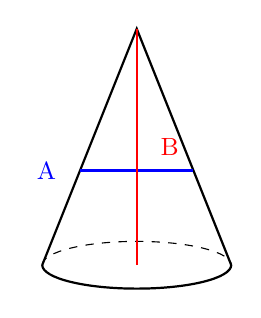
\begin{tikzpicture}[scale=0.6]
  % Cone
  \draw[thick] (-2,0) -- (0,5) -- (2,0);
  \draw[thick] (-2,0) arc[start angle=180,end angle=360,x radius=2,y radius=0.5];
  \draw[dashed] (-2,0) arc[start angle=180,end angle=0,x radius=2,y radius=0.5];
  % Cut A - horizontal
  \draw[thick,blue] (-1.2,2) -- (1.2,2);
  \node[left,blue] at (-1.5,2) {\small A};
  % Cut B - vertical through apex
  \draw[thick,red] (0,0) -- (0,5);
  \node[right,red] at (0.3,2.5) {\small B};
\end{tikzpicture}
\end{center}
\end{questionText}
\choiceA{Cut A (horizontal)}
\choiceB{Cut B (vertical through apex)}
\choiceC{Both cuts}
\choiceD{Neither cut}
\correctAnswer{A}
\explanation{Cut A (horizontal, parallel to the base) produces a circle. Cut B (vertical through the apex) produces a triangle.}
\end{practiceQuestion}

\begin{practiceQuestion}{6-6-q09}{mc}
\begin{questionText}
An angle is $4$ times its supplement. What is the angle?
\end{questionText}
\choiceA{$36°$}
\choiceB{$45°$}
\choiceC{$120°$}
\choiceD{$144°$}
\correctAnswer{D}
\explanation{Let the supplement be $x$. The angle is $4x$. Sum: $x + 4x = 180$. So $5x = 180$ and $x = 36°$. The angle: $4(36) = 144°$.}
\end{practiceQuestion}

\begin{practiceQuestion}{6-7-q17}{mc}
\begin{questionText}
Point $M(3, -5)$ is reflected over the $x$-axis and then over the $y$-axis. What are the final coordinates?
\end{questionText}
\choiceA{$(3, 5)$}
\choiceB{$(-3, -5)$}
\choiceC{$(-3, 5)$}
\choiceD{$(3, -5)$}
\correctAnswer{C}
\explanation{Over $x$-axis: $(3, -5) \to (3, 5)$. Over $y$-axis: $(3, 5) \to (-3, 5)$.}
\end{practiceQuestion}

\begin{practiceQuestion}{7-3-q11}{mc}
\begin{questionText}
A circular rug has a diameter of $8$ feet. What is the area of the rug? Use $\pi \approx 3.14$.
\end{questionText}
\choiceA{$25.12$ ft$^2$}
\choiceB{$50.24$ ft$^2$}
\choiceC{$200.96$ ft$^2$}
\choiceD{$64$ ft$^2$}
\correctAnswer{B}
\explanation{$r = 8 \div 2 = 4$ ft. $A = \pi r^2 = 3.14 \times 16 = 50.24$ ft$^2$.}
\end{practiceQuestion}

\begin{practiceQuestion}{7-4-q16}{mc}
\begin{questionText}
A figure is made of a right triangle with legs $6$ cm and $8$ cm, and a rectangle $8$ cm by $3$ cm. What is the total area?
\end{questionText}
\choiceA{$24$ cm$^2$}
\choiceB{$48$ cm$^2$}
\choiceC{$36$ cm$^2$}
\choiceD{$72$ cm$^2$}
\correctAnswer{B}
\explanation{Triangle: $\frac{1}{2} \times 6 \times 8 = 24$ cm$^2$. Rectangle: $8 \times 3 = 24$ cm$^2$. Total: $24 + 24 = 48$ cm$^2$.}
\end{practiceQuestion}

\begin{practiceQuestion}{7-5-q29}{gsa}
\begin{questionText}
The net shown below folds into a rectangular prism. Find the total surface area.

\begin{center}
\begin{tikzpicture}[scale=0.35]
  \draw[thick,funBlue,fill=funBlue!10] (0,0) rectangle (10,4);
  \draw[thick,funBlue,fill=funBlue!10] (10,0) rectangle (14,4);
  \draw[thick,funBlue,fill=funBlue!10] (14,0) rectangle (24,4);
  \draw[thick,funBlue,fill=funBlue!10] (24,0) rectangle (28,4);
  \draw[thick,funBlue,fill=funBlue!10] (0,4) rectangle (10,8);
  \draw[thick,funBlue,fill=funBlue!10] (0,-4) rectangle (10,0);
  % Dimensions
  \draw[thick,funRed,<->] (0,-5) -- (10,-5);
  \node[below,funRed] at (5,-5) {$10$ cm};
  \draw[thick,funRed,<->] (10,-5) -- (14,-5);
  \node[below,funRed] at (12,-5) {$4$};
  \draw[thick,funRed,<->] (-1,0) -- (-1,4);
  \node[left,funRed] at (-1,2) {$4$ cm};
\end{tikzpicture}
\end{center}
\end{questionText}
\correctAnswer{$192$ cm$^2$}
\explanation{The prism is $10 \times 4 \times 4$. $SA = 2(10 \times 4) + 2(10 \times 4) + 2(4 \times 4) = 80 + 80 + 32 = 192$ cm$^2$.}
\end{practiceQuestion}

\begin{practiceQuestion}{7-6-q18}{mc}
\begin{questionText}
A trapezoidal prism has a trapezoidal base with parallel sides $4$ cm and $6$ cm, height $3$ cm, and the prism length is $10$ cm. What is its volume?
\end{questionText}
\choiceA{$60$ cm$^3$}
\choiceB{$120$ cm$^3$}
\choiceC{$150$ cm$^3$}
\choiceD{$180$ cm$^3$}
\correctAnswer{C}
\explanation{$B = \frac{1}{2}(4 + 6) \times 3 = 15$ cm$^2$. $V = 15 \times 10 = 150$ cm$^3$.}
\end{practiceQuestion}

\begin{practiceQuestion}{8-1-q12}{mc}
\begin{questionText}
Which of the following increases the reliability of conclusions drawn from a sample?
\end{questionText}
\choiceA{Using a smaller sample}
\choiceB{Using a larger random sample}
\choiceC{Surveying only people who agree with you}
\choiceD{Using a non-random sample}
\correctAnswer{B}
\explanation{Larger random samples better represent the population and give more reliable results.}
\end{practiceQuestion}

\begin{practiceQuestion}{8-3-q18}{mc}
\begin{questionText}
School A: median score $88$, MAD $4$. School B: median score $82$, MAD $4$. The difference in medians expressed in MADs is:
\end{questionText}
\choiceA{$1$ MAD}
\choiceB{$1.5$ MADs}
\choiceC{$2$ MADs}
\choiceD{$4$ MADs}
\correctAnswer{B}
\explanation{Difference in medians: $88 - 82 = 6$. In MADs: $\frac{6}{4} = 1.5$ MADs.}
\end{practiceQuestion}

\begin{practiceQuestion}{8-4-q22}{sa}
\begin{questionText}
Group X: mean $45$, MAD $6$. Group Y: mean $57$, MAD $6$. Express the difference in means as a multiple of MAD.
\end{questionText}
\correctAnswer{$2$ MADs}
\explanation{Difference: $57 - 45 = 12$. In MADs: $\frac{12}{6} = 2$.}
\end{practiceQuestion}

\begin{practiceQuestion}{8-7-q18}{mc}
\begin{questionText}
Which statement is true about frequency tables?
\end{questionText}
\choiceA{They only work for numerical data}
\choiceB{They can organize both categorical and numerical data}
\choiceC{They always require intervals}
\choiceD{They show data as a graph}
\correctAnswer{B}
\explanation{Frequency tables can list categories (favorite color) or numerical intervals (test scores $70$--$79$).}
\end{practiceQuestion}

\begin{practiceQuestion}{9-4-q03}{mc}
\begin{questionText}
A bag contains $4$ red marbles and $1$ blue marble. Which type of probability model does this represent?
\end{questionText}
\choiceA{Uniform}
\choiceB{Non-uniform}
\choiceC{Both uniform and non-uniform}
\choiceD{Neither}
\correctAnswer{B}
\explanation{The probability of drawing red ($\frac{4}{5}$) is different from drawing blue ($\frac{1}{5}$), so this is a non-uniform model.}
\end{practiceQuestion}

\begin{practiceQuestion}{9-6-q04}{mc}
\begin{questionText}
Two dice are rolled. What is the probability of getting a sum of $2$?
\end{questionText}
\choiceA{$\frac{1}{6}$}
\choiceB{$\frac{1}{12}$}
\choiceC{$\frac{1}{36}$}
\choiceD{$\frac{2}{36}$}
\correctAnswer{C}
\explanation{The only way to get a sum of $2$ is $(1,1)$. $P = \frac{1}{36}$.}
\end{practiceQuestion}

\begin{practiceQuestion}{9-7-q15}{mc}
\begin{questionText}
You simulate flipping a coin $3$ times and counting how many times all $3$ are heads. In $40$ simulations, all $3$ heads occurs $6$ times. What is the experimental probability?
\end{questionText}
\choiceA{$\frac{6}{40} = 0.15$}
\choiceB{$\frac{1}{8} = 0.125$}
\choiceC{$\frac{3}{40} = 0.075$}
\choiceD{$\frac{6}{120} = 0.05$}
\correctAnswer{A}
\explanation{$P = \frac{6}{40} = 0.15$. The theoretical probability is $\frac{1}{8} = 0.125$, close to the simulation result.}
\end{practiceQuestion}
